\documentclass[5p,times]{elsarticle}
% FGCS: elsarticle with 5p,times (FGCS Author Information Pack, 7 Jan 2023); numbered references.
\usepackage[T1]{fontenc}
\usepackage{amsmath,amssymb,amsthm}
\usepackage{booktabs}
\usepackage{microtype}
\setlength{\emergencystretch}{1.5em}
\usepackage{enumitem}
\usepackage{xcolor}
\usepackage{tikz}
\usetikzlibrary{arrows.meta,positioning}
\usepackage{pgfplots}
\pgfplotsset{compat=1.18}
\usepackage{algorithm}
\usepackage[noend]{algpseudocode}
\usepackage[hidelinks]{hyperref}
\usepackage[capitalise,nameinlink]{cleveref}

\newtheorem{proposition}{Proposition}
\newtheorem{remark}{Remark}
\crefname{remark}{Remark}{Remarks}
\crefname{proposition}{Proposition}{Propositions}
\crefname{algorithm}{Algorithm}{Algorithms}
\crefname{equation}{Eq.}{Eqs.}

% Draft markers: must be empty before submission (checked by audit scan).
\DeclareRobustCommand{\authorfield}[1]{\textcolor{red!70!black}{[#1]}}

\journal{Future Generation Computer Systems}

\begin{document}

\begin{frontmatter}

\title{Green Shaping: Energy-Aware Design and Validation of Metadata Protection for LLM-Orchestrated Federated Analytics}

% Author names link to the ORCID records supplied by the corresponding team.
\author[aff1]{\mbox{\href{https://orcid.org/0000-0003-0991-6157}{Lam Nguyen Tran Thanh}}}
\ead{thanhlam.bk.2110@gmail.com}
\author[aff2]{\mbox{\href{https://orcid.org/0000-0002-5674-7985}{Thanh Pham Chi}}}
\ead{thanh.pham@rmit.edu.vn}
\author[aff3]{\mbox{\href{https://orcid.org/0000-0002-5336-0566}{Son Ha Xuan}}}
\ead{ha.son@rmit.edu.vn}
\author[aff4]{\mbox{\href{https://orcid.org/0000-0001-9152-6208}{Nguyen Ngoc Phien}}\corref{cor1}}
\ead{nguyenngocphien@tdtu.edu.vn}
\author[aff5]{\mbox{\href{https://orcid.org/0009-0000-2881-0943}{Vo Hong Khanh}}}
\ead{khanhvh@fe.edu.vn}
\author[aff5]{\mbox{\href{https://orcid.org/0009-0009-4235-584X}{Nguyen Minh Triet}}}
\ead{trietnm3@fe.edu.vn}
\author[aff6]{\mbox{\href{https://orcid.org/0009-0009-0116-1619}{Duy Pham Dang Xuan}}}
\ead{duy25msa23258@fsb.edu.vn}
\author[aff6]{\mbox{\href{https://orcid.org/0009-0003-5046-5535}{Tung Nguyen Quang}}}
\ead{NguyenQuangTung0902@gmail.com}
\cortext[cor1]{Corresponding author.}
\address[aff1]{Ho Chi Minh City University of Technology and Engineering, 01 Vo Van Ngan Street, Thu Duc Ward, Ho Chi Minh City, Vietnam}
\address[aff2]{Electronic and Computer Systems Engineering (SSET), RMIT, SGS campus, Vietnam}
\address[aff3]{Digital Economy, The Business School (TBS), RMIT, Ho Chi Minh City, Vietnam}
\address[aff4]{Center for Applied Information Technology and Faculty of Information Technology, Ton Duc Thang University, Ho Chi Minh City, Vietnam}
\address[aff5]{FPT University, Cantho Campus, Vietnam}
\address[aff6]{FPT University, Ho Chi Minh City Campus, Vietnam}

\begin{abstract}
An LLM planner can turn an analyst's question into federated tool calls, whose encrypted traffic still exposes sizes, timing and participation metadata. Protecting that metadata consumes resources at data sites, including sites sending only cover traffic. We present Green Shaping, an energy-aware design combining bucketed padding, synchronised rounds with cover sites and fixed-tick differentially private byte release. The analysis bounds padded-size information, establishes a per-site energy floor for hiding participation, scopes the release guarantee under feedback and derives its padding cost; the queue-length variant has quadratic tick-count growth at a fixed privacy budget. An energy-budgeted controller is formulated with symbolic per-node costs. We evaluate the implementation on a projection of public HIGGS data using 20 logical partitions. Functional/cost calibration completes 360 TRAIN and 216 SELECT trials, retaining 12 failures, while two local LLMs pass 48 repaired typed-plan and structured-summary checks. A four-instance EC2 deployment completes 168 reference-correct three-step-workflow sessions across seven modes, with matched network captures and replicated evidence. The evaluation reports network bytes, latency, correctness and recovery integrity. Retrospective classifiers probe leakage; public-contract bounds, synthetic admission tests and paired loopback TLS experiments expose reliability and resource limits. Physical joules and edge performance remain unmeasured; no empirical privacy-per-joule optimum is established. The results expose substantial framing and DP release costs and provide a reproducible basis for later instrumented privacy--energy evaluation.
\end{abstract}

\begin{keyword}
federated analytics \sep LLM agents \sep traffic analysis \sep traffic shaping \sep differential privacy \sep energy efficiency
\end{keyword}

\end{frontmatter}

\section{Introduction}\label{sec:intro}

Federated analytics computes statistics across institutions without moving raw data to a central place~\cite{wang2022federated,elkordy2023federated}. A recent line of systems puts a large language model (LLM) agent in charge of planning such analyses: LAFA, which its authors describe as ``the first system that integrates LLM-agent-based data analytics with FA'', turns natural-language queries into optimised federated-analytics workflows~\cite{ji2025lafa}, agent frameworks such as LangGraph orchestrate stateful agents~\cite{langgraph2026docs}, and tool protocols such as the Model Context Protocol carry each tool message as an HTTP request~\cite{mcp2026spec}. In this paper we consider the tool-calling form of this design: an orchestrating agent turns an analyst's question into tool calls to data sites and aggregates their replies.

Encryption protects the content of each call and reply but does not hide its length~\cite{rfc9846}, and its timing is visible to any on-path observer. Traffic analysis has repeatedly shown that such metadata is enough to infer what a user is doing: which web page is loaded~\cite{panchenko2016website,sirinam2018deep}, what an AI assistant is answering~\cite{weiss2024what,mcdonald2025whisper}, which LLM agent a user is running and for which task~\cite{zhang2025agentprint,pouryousef2026benchmark}, and which model architecture a federated-learning client trains~\cite{shuvo2025flare,shuvo2026flint}. In agent-orchestrated federated analytics the same observer, placed on the links between the orchestrator and the sites, sees which sites are called and the size and timing of every exchange, which may reveal how much data each site processes and what kind of query runs. In cross-institution health or finance analytics, participation and data volume can be sensitive on their own.

Padding, batching and differentially private shaping can hide this metadata~\cite{cai2014systematic,wang2017walkie,sabzi2024netshaper}, but they are not free. Every padded byte is sent and received, every cover message wakes a node, and a shaper that releases data at fixed ticks keeps nodes active. On edge devices and in large server deployments the energy adds up, and the cost of anonymity traffic has already been shown to be material on smartphones~\cite{hugenroth2023powering}. Sustainable data infrastructure needs to know what metadata protection costs in joules, and operators need a way to spend a fixed energy budget where it reduces leakage most. Energy-constrained cover traffic has a long history in sensor-network location privacy~\cite{kamat2005enhancing,shao2008towards}, but our search found no work that studies orchestrator-to-site metadata in agentic federated analytics or evaluates its defences under an energy budget (\cref{sec:related}).

We present \emph{Green Shaping}. It shapes traffic at the tool-call layer, where whole calls and replies are visible before encryption, with three primitives: bucketed padding, synchronised rounds with cover sites, and a differentially private (DP) release of queued bytes at fixed ticks in the style of NetShaper~\cite{sabzi2024netshaper}. We formulate a controller that would choose the primitives' parameters from a calibrated per-node energy model and an attacker retrained on shaped traffic, subject to a joule budget per node. The completed implementation study evaluates correctness and observable resource costs; it does not validate a joule-constrained privacy optimum.

The contributions combine a scoped design and analysis with a reproducible engineering evaluation:
\begin{enumerate}[label=(\arabic*),leftmargin=*,noitemsep,topsep=2pt]
\item A system and threat model for passive inference of site participation, contribution size and query family from orchestrator-to-site metadata (\cref{sec:model}).
\item The Green Shaping design: three tool-call-layer primitives, the deployment conditions they need, a per-node energy cost model and a budget-constrained selection algorithm, with a reference implementation (\cref{sec:design}).
\item An analysis that scopes what each primitive can and cannot guarantee (\cref{sec:analysis}): a bound on the information a padded message size can carry; an energy floor at every site for hiding participation, so that the network-wide cost grows with the number of sites; a DP guarantee for the release mechanism under feedback between links, with a bound on any attacker's accuracy and an exact expression for its padding cost, which for the queue-length release grows with the square of the number of ticks; and the order in which primitives must be combined.
\item A bounded implementation study on public HIGGS data: TRAIN/SELECT calibration over 20 logical partitions, typed-plan and numerical-summary validation with two local LLMs, and 168 successful sessions through a four-instance EC2 deployment with captures at both sides of a common observer link (\cref{sec:eval,sec:results}). The study measures correctness, bytes, latency and recovery integrity, with retrospective question-disjoint metadata classification and independently validated fixed-arrival stress tests. It does not measure physical joules or edge-device performance, or establish a final-test privacy ranking.
\item A public-contract completion bound and prototype admission layer with per-node modelled budgets. Synthetic deployment and workflow-envelope studies compare conservative tick accounting, occupied-tick accounting, public clipping and constant cover. Paired loopback TLS acquisition additionally tests the envelope against two periodic-cover frequencies (\cref{sec:admission,sec:stress,sec:localtls}). Multi-host validation of these new candidates remains open.
\end{enumerate}

\Cref{sec:related} reviews related work. \Cref{sec:model,sec:design,sec:analysis} present the model, design and analysis. \Cref{sec:eval,sec:results} give the methodology and measured results, \cref{sec:discussion} discusses implications and limitations, and \cref{sec:conclusion} concludes.

\section{Background and related work}\label{sec:related}

\subsection{Federated analytics and agent orchestration}
Federated analytics (FA) performs data analytics across decentralised parties while raw data stays local; unlike federated learning, its goal is to draw conclusions from data rather than to train a model~\cite{wang2022federated}. Surveys cover its query types and its use across devices and institutional silos such as hospitals and banks~\cite{elkordy2023federated,wang2024survey}. Privacy in FA is usually framed around intermediate and released results and handled with secure computation, homomorphic encryption and differential privacy~\cite{wang2022federated}, the latter in the sense of~\cite{dwork2014algorithmic}; traffic metadata is not discussed there. LAFA adds a hierarchy of LLM agents that turns natural-language queries into workflow graphs, which an existing FA backend executes with encryption and output DP~\cite{ji2025lafa}. Agentic orchestration of federated learning has also been proposed~\cite{jarczewski2026agentic}. Our system model differs from LAFA in that the agent calls sites directly as tools, as frameworks such as LangGraph~\cite{langgraph2026docs} and the Model Context Protocol, whose Streamable HTTP transport sends each message as an HTTP POST~\cite{mcp2026spec}, make possible; the coordination traffic is then a sequence of encrypted calls and replies per site. Surveys of LLM-agent security cover threats ranging from prompt injection to protocol exploits~\cite{deng2025agents,ferrag2026prompt}.

\subsection{Traffic analysis of encrypted traffic, LLM services and agents}
Website fingerprinting showed early that encryption does not hide what a user loads: packet sizes and directions identify pages~\cite{panchenko2016website}, and deep classifiers exceed 98\% accuracy on undefended Tor traffic~\cite{sirinam2018deep}. Dyer et al.\ showed that nine countermeasures, including per-packet padding, fail against attacks on coarse features such as total time and bandwidth~\cite{dyer2012peekaboo}. LLM services leak through the same channel. Streaming responses reveal token lengths, from which 27\% of responses were reconstructed and 53\% had their topic inferred~\cite{weiss2024what}; record sizes and timing of streamed responses reveal prompt topics across 28 models~\cite{mcdonald2025whisper}; efficient inference creates data-dependent timing~\cite{carlini2024remote} and speculative decoding leaks through packet sizes~\cite{wei2024speculation}; and deployed provider padding still leaves substantial leakage~\cite{zhang2025netecho}. For agents, AgentPrint identifies which of 50 agents a user runs from encrypted user-to-cloud traffic with a CNN on time-sliced packet counts and volumes, and infers user occupation from agent use~\cite{zhang2025agentprint}. Pouryousef et al.\ fingerprint multi-agent tasks from agent-to-LLM traffic with a random forest at up to 90.7\% accuracy, without observing tool traffic~\cite{pouryousef2026benchmark}. MCP traffic has regular, beacon-like timing~\cite{sohail2026beacons}. None of these works observes the links between an orchestrator and data sites, or targets participation and data volume.

\subsection{Side channels in federated systems}
On federated learning, FLARE infers the model-architecture family of clients from encrypted Wi-Fi traffic with random forests~\cite{shuvo2025flare}, FLINT does so from 5G physical-layer scheduling metadata~\cite{shuvo2026flint}, and network traffic patterns identify client architectures on an FL testbed~\cite{shuvo2025fingerprinting}. FL flows themselves are identifiable from their first packets~\cite{boiano2024first}. These works infer what model is trained or whether FL is used; they do not infer which sites take part in an analysis or how much data each contributes, and they evaluate no defence with its energy cost.

\subsection{Shaping defences and their cost}
Constant-rate and burst-based defences trade bandwidth and latency for protection: Tamaraw pads to fixed packet sizes and rates~\cite{cai2014systematic}, CS-BuFLO adapts constant-rate shaping to congestion~\cite{cai2014csbuflo}, WTF-PAD and FRONT add dummy packets, FRONT with zero added latency~\cite{juarez2016toward,gong2020zero}, and Walkie-Talkie moulds bursts at 31\% bandwidth and 34\% time overhead~\cite{wang2017walkie}. Pacer shapes cloud traffic secret-independently in the hypervisor~\cite{mehta2022pacer}. Differentially private shaping gives formal guarantees: Zhang et al.\ apply DP to the byte time series of streaming traffic, including an offline Fourier-based mechanism~\cite{zhang2019statistical}, Xiong et al.\ propose an event-level DP shaper for IoT streams~\cite{xiong2021traffic}, and NetShaper releases a Gaussian-noised amount of queued data per fixed interval from a middlebox tunnel, with window-based adjacency and R\'enyi DP accounting~\cite{sabzi2024netshaper}. For LLM traffic, random padding, token batching and packet injection each reduce but do not remove leakage, the last at two to three times the traffic volume~\cite{mcdonald2025whisper}. Worae et al.\ shape IoT traffic under bandwidth and latency budgets~\cite{worae2026adaptive}. Energy has been a design constraint mainly in sensor networks, where source-location privacy against eavesdroppers was traded against transmission cost: phantom routing was evaluated by its energy cost against flooding and fake sources~\cite{kamat2005enhancing}, and dummy messages at statistically shaped intervals hide real events from a global observer at a message overhead that sensors' limited energy forces to stay low~\cite{shao2008towards}. In general-purpose networks, Hugenroth and Beresford measured that a mix-network client with continuous cover traffic costs up to 24 percentage points of smartphone battery over 12 hours~\cite{hugenroth2023powering}, and mobile measurements show that network energy depends on the transfer pattern, not only on bytes, because of radio tail states~\cite{balasubramanian2009energy,huang2012close}.

\subsection{Energy measurement and reporting}
Intel RAPL counters track package power closely but update about every millisecond, wrap around and need careful sampling~\cite{khan2018rapl}; DRAM readings can deviate substantially near idle~\cite{desrochers2016validation}; and RAPL polling tools add overhead~\cite{diamond2026cost}. The Linux powercap interface exposes the counters as cumulative microjoule values with their wrap-around range~\cite{linux2026powercap}. Internal power sensors on Jetson devices can underestimate power by up to 50\% without calibration~\cite{shalavi2023accurate}, which favours external meters. Work on sustainable machine learning asks that energy and carbon be reported systematically~\cite{henderson2020towards,patterson2021carbon,lacoste2019quantifying} and computed from location- and time-specific grid intensity~\cite{dodge2022measuring}.

\subsection{Positioning}
\Cref{tab:related} summarises the closest work. Our search, through 18 October 2026, found no work that targets orchestrator-to-site metadata in agentic federated analytics, and none that combines padding, cover traffic and DP shaping under a per-node energy budget in that setting. Its individual primitives are not new: padding, batching, cover traffic and DP shaping all exist. Nor is energy-constrained cover traffic new~\cite{kamat2005enhancing,shao2008towards,hugenroth2023powering}. The contribution lies in the threat setting, in the analysis of what each primitive can achieve and cost there, in their energy-budgeted combination, and in the measurement methodology.

\begin{table*}[t]
\centering
\caption{Closest prior work. Vantage: where the observer sits. ``none'': not addressed.}\label{tab:related}
\footnotesize
\begin{tabular}{@{}p{2.5cm}p{2.5cm}p{3.1cm}p{3.1cm}p{2.0cm}p{2.3cm}@{}}
\toprule
Work & Vantage & Inferred secret & Defence evaluated & Formal guarantee & Energy measured \\
\midrule
AgentPrint~\cite{zhang2025agentprint} & user to cloud agent & agent, behaviour, occupation & none (discussed) & none & none \\
Pouryousef et al.~\cite{pouryousef2026benchmark} & agent to LLM & model, prompt category, multi-agent task & prompt reformulation, temperature & none & none \\
Whisper Leak~\cite{mcdonald2025whisper} & user to LLM & prompt topic & padding, batching, injection & none & none \\
FLARE, FLINT~\cite{shuvo2025flare,shuvo2026flint} & FL client link (Wi-Fi, 5G PHY) & model architecture & none & none & none \\
NetShaper~\cite{sabzi2024netshaper} & network middlebox & web/video content & DP shaping & $(\varepsilon,\delta)$-DP & none \\
Worae et al.~\cite{worae2026adaptive} & IoT device & device fingerprint & budgeted camouflage & none & none (bandwidth, latency) \\
Hugenroth and Beresford~\cite{hugenroth2023powering} & smartphone & none & Tor, mix network cover traffic & none & yes (battery) \\
LAFA~\cite{ji2025lafa} & none & none & output DP & output DP & none \\
\midrule
This paper & orchestrator to sites & participation, size, query family & padding, rounds with cover sites, DP release & $\varepsilon$-DP (DP release) & planned (RAPL, meters) \\
\bottomrule
\end{tabular}
\end{table*}

\section{System and threat model}\label{sec:model}

\subsection{Agent-orchestrated federated analytics}
A deployment has one orchestrator $O$ and $N$ data sites $S_1,\dots,S_N$ (\cref{fig:arch}). An analyst submits a natural-language question to $O$. An LLM agent at $O$ plans the analysis and issues \emph{tool calls}, one HTTP request to one site endpoint each, carrying a query or a model update. Each site runs the request on its local data and returns a \emph{reply} with a partial result: an aggregate, a grouped table, a model update or a count. The agent may run several rounds before it aggregates the replies and answers. We call all calls and replies caused by one question a \emph{session}. Every orchestrator-site link uses TLS and a persistent connection, so payloads and headers are encrypted.

\begin{figure}[t]
\centering
\resizebox{\columnwidth}{!}{%
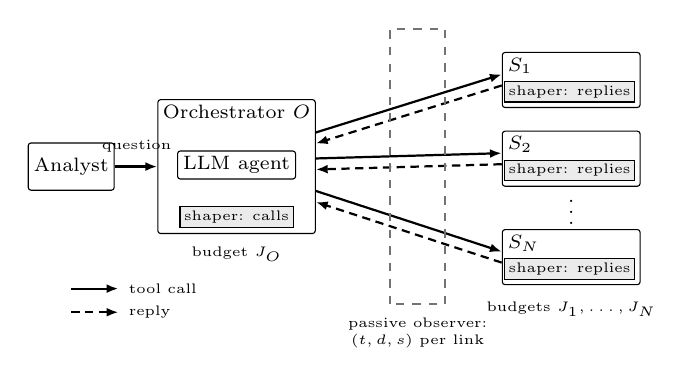
\begin{tikzpicture}[
  font=\scriptsize,
  box/.style={draw, rounded corners=1pt, align=center, inner sep=2pt},
  shp/.style={draw, fill=black!8, align=center, inner sep=1.5pt, font=\tiny},
  call/.style={-{Latex[length=1.5mm]}, thick},
  reply/.style={-{Latex[length=1.5mm]}, thick, densely dashed}]
\node[box, minimum width=0.95cm, minimum height=0.6cm] (an) at (0,0) {Analyst};
\node[box, minimum width=2.0cm, minimum height=1.7cm] (orch) at (2.1,0) {};
\node[anchor=north, inner sep=2pt] at (orch.north) {Orchestrator $O$};
\node[box, fill=white] at ([yshift=0.02cm]orch.center) {LLM agent};
\node[shp, anchor=south] at ([yshift=0.08cm]orch.south) {shaper: calls};
\draw[call] (an.east) -- (orch.west);
\node[font=\tiny, anchor=south] at (0.83,0.06) {question};
\foreach \y/\n/\lab in {1.1/1/S_1, 0.1/2/S_2, -1.15/3/S_N} {
  \node[box, minimum width=1.75cm, minimum height=0.7cm] (s\n) at (6.35,\y) {};
  \node[anchor=north west, inner sep=2pt] at (s\n.north west) {$\lab$};
  \node[shp, anchor=south east] at ([xshift=-0.07cm, yshift=0.07cm]s\n.south east) {shaper: replies};
  \draw[call]  ([yshift=0.07cm+0.33*\y cm]orch.east) -- ([yshift=0.07cm]s\n.west);
  \draw[reply] ([yshift=-0.07cm]s\n.west) -- ([yshift=-0.07cm+0.33*\y cm]orch.east);
}
\node at (6.35,-0.48) {$\vdots$};
\draw[dashed, thick, black!55] (4.05,-1.75) rectangle (4.75,1.75);
\node[font=\tiny, align=center, anchor=north] at (4.4,-1.8) {passive observer:\\$(t,d,s)$ per link};
\node[font=\tiny, anchor=north] at (2.1,-0.9) {budget $J_O$};
\node[font=\tiny, anchor=north] at (6.35,-1.6) {budgets $J_1,\dots,J_N$};
\draw[call] (0.0,-1.55) -- (0.6,-1.55) node[right, font=\tiny] {tool call};
\draw[reply] (0.0,-1.85) -- (0.6,-1.85) node[right, font=\tiny] {reply};
\end{tikzpicture}}

\caption{System and threat model. The LLM agent at the orchestrator sends tool calls to sites and receives replies over encrypted links. A passive observer on the links between the orchestrator and the sites records the time, direction and size of every message on every link. Green Shaping runs at the tool-call layer of the orchestrator and at the reply layer of each site, under a per-node joule budget. Drawn as TikZ code prepared with AI assistance (Claude, Anthropic; see the generative AI declaration).}
\label{fig:arch}
\end{figure}

\subsection{Observer}
The adversary is passive and sits on the network between $O$ and the sites, for example on a shared data-centre fabric, an institutional uplink or a wide-area segment. For every link $i$ it records the sequence of messages $(t,d,s)$ with time $t$, direction $d\in\{\uparrow,\downarrow\}$ (call or reply) and size $s$ in bytes. It groups packets into application messages by inter-packet gaps, which needs no decryption. It cannot decrypt traffic, compromise $O$ or a site, inject or delay packets, or see the analyst's question. It knows the system design, the set of sites, the shaping mechanism and its parameters, and it can collect labelled training traffic from a replica of the deployment (Kerckhoffs' principle). It retrains on traffic shaped with the configuration under test, so a complete empirical privacy evaluation would require an attacker adapted to each defence. The retrospective diagnostic retrains a fixed classifier under each mode on the multiplexed observer link; it does not constitute a confirmatory per-site evaluation of this stronger observer.

\subsection{Secrets}
Per session the observer tries to infer three properties:
\begin{enumerate}[label=(\roman*),noitemsep,topsep=2pt]
\item \emph{participation}: whether site $i$ was called, which reveals that it holds data relevant to the question;
\item \emph{contribution size}: the size bucket of the data that site $i$ processed, a proxy for how many records it holds that match the query;
\item \emph{query family}: aggregate statistics, group-by, a training job, or a record count.
\end{enumerate}
Which channel carries contribution size depends on the query: for group-by queries and training rounds it may appear in reply sizes, while for aggregates and counts the reply size is fixed and only the time a site takes to answer may depend on its data. In cross-institution health or finance analytics these properties can be sensitive on their own: participation in a study on a rare condition, or the volume of matching records at one institution, can disclose information that the payload encryption was meant to protect.

\subsection{Assumptions and scope}
Sites and orchestrator are honest and follow the protocol. The energy-budget design assumes that a deployment can calibrate energy costs; the EC2 validation does not supply those measurements. The study covers one orchestrator and direct calls to sites. It does not cover chains of agents, compromised sites, active traffic manipulation, or the privacy of the analytics result itself, which needs output-level protection such as differential privacy on the released statistic~\cite{dwork2014algorithmic} and is orthogonal to the coordination metadata studied here. Traffic between the orchestrator and a hosted LLM API is also out of scope; an observer of that link can infer task structure~\cite{pouryousef2026benchmark}, which a locally served model avoids.

\section{Green Shaping}\label{sec:design}

Green Shaping has three shaping primitives and a controller that chooses their parameters under a joule budget for each node. \Cref{tab:notation} lists the notation used here and in \cref{sec:analysis}.

\begin{table}[t]
\centering
\caption{Notation.}\label{tab:notation}
\footnotesize
\begin{tabular}{@{}ll@{}}
\toprule
Symbol & Meaning \\
\midrule
$N$; $i$ & number of sites; site and link index \\
$\beta$, $r$ & padding base (bytes) and bucket ratio ($r>1$) \\
$W$, $R$ & batching round length (s); reply frame size (bytes) \\
$q_i$ & probability that site $i$ is a cover site in a session \\
$\tau$, $K$, $H$ & DP tick length, ticks per session, $K=\lceil H/\tau\rceil$ \\
$\Delta$ & adjacency bound on bytes entering the DP release \\
$\varepsilon_{\mathrm{dir}}$, $\varepsilon_w$ & budget per link-direction; per tick, $\varepsilon_w=\varepsilon_{\mathrm{dir}}/K$ \\
$a_k$, $Q_k$, $b_k$ & bytes arriving, queued and released at tick $k$ \\
$L_k$ & Laplace noise drawn at tick $k$ \\
$\theta$; $\Theta\supseteq\Theta_1$ & configuration; grid; single-primitive subset \\
$\mathcal{F}(\cdot)$ & configurations within budget and without overflow \\
$\hat A(\theta)$ & attacker advantage on the selection questions \\
$E^{\mathrm{raw}}_n$, $\hat E_n$ & modelled energy; extra energy over unshaped (J) \\
$J_n$ & joule budget of node $n$ per session (J) \\
$e_{\mathrm{tx}}$, $e_{\mathrm{rx}}$ & energy per byte sent and received (J/B) \\
$p_{\mathrm{aw}}$, $t_{\mathrm{tail}}$ & active power above idle (W); activity tail (s) \\
$\pi_i$, $\alpha$ & prior of participation; target detector accuracy \\
$e_{\min,i}$ & minimum extra energy of site $i$ to act as cover in a session \\
\bottomrule
\end{tabular}
\end{table}

\subsection{Placement at the tool-call layer}
The shaper wraps the tool client in the orchestrator and the tool server at each site. At this layer it sees whole calls and replies, knows which session they belong to and knows the full set of sites, information that a packet-level shaper in a middlebox has to infer or does without. It shapes application messages before TLS encryption, so padding and cover messages are encrypted like real traffic and cannot be told apart by content. Tool interfaces such as the Model Context Protocol~\cite{mcp2026spec} define a request and response unit, which gives padding and batching a natural hook. The DP release needs more: it sends a scheduled byte stream, so it runs over one long-lived framed connection per link beneath the tool-call interface (\cref{sec:deploy}). Whether shaping at this layer is cheaper than packet-level shaping at equal attacker advantage is an open empirical question. Our NetShaper comparison measures functional and network costs, not matched privacy.

\subsection{Primitives}

\paragraph{Bucketed padding} Every call and reply body is padded to the next size in a geometric ladder: a message of $m$ bytes becomes
\begin{equation}\label{eq:pad}
\mathrm{pad}(m)=\begin{cases}\beta, & m\le\beta,\\ \beta\, r^{\lceil \log_r (m/\beta)\rceil}, & m>\beta.\end{cases}
\end{equation}
Padding is added inside the encrypted body. The ratio $r$ trades bytes for the number of distinguishable size classes (\cref{prop:pad}). Padding changes neither the number of messages nor their timing.

\paragraph{Synchronised rounds with cover sites} At the start of a session, each site that the agent will not call is made a \emph{cover site} with probability $q_i$; the decision holds for the whole session. Called sites and cover sites form the \emph{active set}. The orchestrator releases calls only at multiples of a round length $W$. At each round boundary every active site receives exactly one call frame, whose size is the round's largest call, padded with \cref{eq:pad}; the orchestrator knows every call it releases, so it can size the frame. Replies travel in frames of a fixed size $R$: every active site sends one frame at the boundary $W$ after the call and, if any reply is incomplete, one more frame per further boundary after a poll from the orchestrator. A called site fills its frames with reply data that is ready; a cover site sends filler. The orchestrator stops polling once every called site has signalled, inside its encrypted frames, that its reply is complete, so all active sites send the same number of frames. Within a session every active link therefore carries the same sequence of times, directions and sizes. What stays visible is the active set, the number of rounds, the call-frame class and the number of reply frames per round, which depends on the largest reply. Rounds cost latency of up to one round per direction and the energy of cover sites, and it removes the per-site timing that otherwise reveals how much work a site performs.

\paragraph{Differentially private release} On each link and direction the shaper keeps a queue and releases bytes only at fixed ticks $k\tau$, $k=1,\dots,K$, for all $N$ sites from the start of the session, independently of the data. At tick $k$ it reads the queue length $Q_k$, draws Laplace noise, and sends exactly
\begin{equation}\label{eq:dp}
b_k=\max\bigl(0,\operatorname{round}(Q_k+L_k)\bigr),\qquad L_k\sim\mathrm{Lap}(\Delta/\varepsilon_w),
\end{equation}
bytes: $\min(Q_k,b_k)$ bytes of queued data followed by padding. $\Delta$ is set on the bytes that enter this primitive, after batching and padding (\cref{prop:order}). This follows the queue-based design of NetShaper~\cite{sabzi2024netshaper}, which noises the amount of data released per fixed interval rather than the send times. NetShaper uses Gaussian noise, adjacency over sliding windows and R\'enyi DP accounting in a middlebox tunnel; we use Laplace noise per link at the end hosts and prove the guarantee for this mechanism directly in \cref{prop:dp} rather than inheriting NetShaper's.

\begin{table*}[t]
\centering
\caption{Where each primitive spends resources and what it protects. Entries are qualitative and follow from the definitions; physical energy coefficients and comparisons across node classes are outside the completed evaluation.}\label{tab:primitives}
\footnotesize
\begin{tabular}{@{}p{2.6cm}p{3.9cm}p{3.6cm}p{2.9cm}p{3.6cm}@{}}
\toprule
Primitive & Extra bytes & Extra awake time & Latency & Guarantee \\
\midrule
Padding & $<(r{-}1)m$ per message if $m>\beta$; $\beta-m$ otherwise & none & none & size classes (\cref{prop:pad}) \\
Rounds with cover sites & frame padding; all traffic of cover sites; polls & cover sites mirror the session; transfers aligned to rounds & up to $W$ per direction and round & equal links within the active set; participation floor (\cref{prop:cover}) \\
DP release & $K\cdot E[\max(0,L_k)]$ per link-direction (\cref{eq:dpcost}) & every tick at every site & queueing, ${\ge}\tau$ & $\varepsilon$-DP (\cref{prop:dp}) \\
\bottomrule
\end{tabular}
\end{table*}

\subsection{Deployment conditions}\label{sec:deploy}
The guarantees of \cref{sec:analysis} hold only if the implementation keeps everything else on the wire independent of the data. (i) \emph{Transport}: each link uses one long-lived TLS connection carrying a framed byte stream (for example an HTTP/2 stream or a WebSocket) on which the tool calls are multiplexed; the DP release writes $b_k$ bytes per tick to this stream. (ii) \emph{Control traffic}: keep-alives, flow-control updates and key updates are disabled during a session or sent on the tick schedule; connection loss aborts the session. (iii) \emph{Session start}: the orchestrator signals the start of a session to all $N$ sites, because a site that starts its ticks only when it is called reveals that it was called; with the DP release every site is therefore active in every session. (iv) \emph{Overflow}: the shaper never sends outside the schedule. A session whose data does not fit in $K$ ticks is truncated and its remaining calls are issued as a new session, which an observer can see; truncations are counted as privacy failures, and $H$ is chosen from calibration sessions to keep them rare. (v) \emph{Concurrency}: sessions on a deployment are serialised; overlapping sessions would need a shared schedule and joint accounting, which we leave open.

\subsection{Energy cost model}
For a shaped session, the controller estimates the energy of node $n$ (a site or the orchestrator) as
\begin{equation}\label{eq:energy}
\begin{aligned}
E^{\mathrm{raw}}_n(\theta)&=e_{\mathrm{tx}}\,B^{\mathrm{tx}}_n+e_{\mathrm{rx}}\,B^{\mathrm{rx}}_n+p_{\mathrm{aw}}\,T^{\mathrm{aw}}_n,\\
\hat E_n(\theta)&=E^{\mathrm{raw}}_n(\theta)-E^{\mathrm{raw}}_n(\varnothing),
\end{aligned}
\end{equation}
where $B^{\mathrm{tx}}_n$ and $B^{\mathrm{rx}}_n$ are the bytes the node sends and receives, $T^{\mathrm{aw}}_n$ is the length of the union of the intervals $[t,t+t_{\mathrm{tail}}]$ over all times $t$ at which the node sends, receives or wakes for a tick, and $\varnothing$ denotes the unshaped session, so $\hat E_n$ is the energy that shaping adds. This is a simple model of a CPU and network interface that stay active for a short time after each transfer. A deployment would fit these four coefficients from instrumented microbenchmarks for its node class. We leave them symbolic: the completed testbed exposes no physical energy counters, so no joule, carbon or measured energy-ranking result is reported (\cref{sec:energy}). The model is a design component, not a fitted empirical predictor in this study. It makes the profiles of the primitives explicit: padding adds only byte terms, rounds add cover traffic but align transfers, and the DP release keeps every node active at every tick.

\subsection{Controller}
\Cref{alg:controller} specifies a proposed energy-budgeted selection procedure, distinct from the functional/cost shortlist used in our implementation study. It selects a configuration offline from sessions recorded on the deployment, split by question into three disjoint sets: attacker training, selection, and a final test set that only the evaluation uses. For each candidate $\theta$ it shapes the sessions, estimates each node's extra energy with \cref{eq:energy}, trains the attacker of \cref{sec:attack} on shaped training sessions and measures its advantage on shaped selection sessions. It returns the feasible configuration with the lowest worst-case advantage over the three secrets. The grid contains every single-primitive configuration, so the selected configuration is never worse on the selection data than the best single primitive within the budget (\cref{rem:dominance}). The controller is rerun when the workload or the budgets change; its cost is $|\Theta|$ shaping passes and attacker trainings.

\begin{algorithm}[t]
\caption{Green Shaping configuration selection}\label{alg:controller}
\footnotesize
\begin{algorithmic}[1]
\Require sessions $\mathcal{C}_{\mathrm{tr}}$, $\mathcal{C}_{\mathrm{sel}}$ with disjoint questions; grid $\Theta\supseteq\Theta_1$; fitted cost models; budgets $(J_n)$
\Ensure configuration $\theta^\star$ or \textsc{infeasible}
\State $\mathcal{F}\gets\emptyset$
\For{$\theta\in\Theta$}
  \State set $\Delta$ of $\theta$ from bytes entering the DP release in $\mathcal{C}_{\mathrm{tr}}\cup\mathcal{C}_{\mathrm{sel}}$
  \State shape $\mathcal{C}_{\mathrm{tr}}$ and $\mathcal{C}_{\mathrm{sel}}$ with $\theta$
  \If{any shaped session overflows} \textbf{continue} \EndIf
  \State $\hat E_n(\theta)\gets$ mean of \cref{eq:energy} over shaped $\mathcal{C}_{\mathrm{sel}}$, for every node $n$
  \If{$\exists n:\hat E_n(\theta)>J_n$} \textbf{continue} \EndIf
  \State train attackers on shaped $\mathcal{C}_{\mathrm{tr}}$
  \State $\hat A(\theta)\gets\max$ over the three secrets of the advantage on shaped $\mathcal{C}_{\mathrm{sel}}$
  \State $\mathcal{F}\gets\mathcal{F}\cup\{\theta\}$
\EndFor
\State \Return $\arg\min_{\theta\in\mathcal{F}}(\hat A(\theta),\max_n \hat E_n(\theta))$ (lexicographic), or \textsc{infeasible} if $\mathcal{F}=\emptyset$
\end{algorithmic}
\end{algorithm}

\subsection{Public-contract admission candidate}\label{sec:admission}
We additionally implement a restricted admission rule using \cref{prop:contract}. Public contracts, risk allocations and policy parameters are frozen before private arrivals. For fixed total privacy budget, we divide $\varepsilon$ among the link-directions and allocate completion risks with total at most $\rho$. A numerical minimax solver distributes these risks to reduce the largest modelled node-cost/budget ratio, using nonnegative node coefficients and the release upper bounds. Every bound and budget is recomputed after solving; failure to admit one candidate is not a proof of global infeasibility. This rule uses analytical privacy and completion certificates rather than the learned attacker objective of Algorithm~\ref{alg:controller}. Expected-cost admission is distinguished from deterministic application-byte admission; neither is a calibrated physical-energy guarantee.

The candidate set must include periodic constant cover. We also implement a public workflow envelope with round cap $R$, planning bound $G$, compute bound $C$ and one-way delivery bound $\ell$. With $T=G+C+2\tau+2\ell$, every site sends a fixed call frame at $u_r=rT+\ell+G+\tau$ and a fixed reply frame at $v_r=(r+1)T$, for $r=0,\ldots,R-1$. Unused sites and rounds still emit cover. Legal bounded calls, computation and planning complete inductively by $RT+\ell$. The abstract frame-metadata transcript is identical across legal private jobs; physical packet timing, TLS behaviour and observable violations require separate validation. Cover must continue after private early completion. We compare this candidate with periodic cover using the same public frame caps, without claiming a new general DP primitive.

\subsection{Reference implementation}
A Python reference implementation provides the three primitives, the cost model, feature extraction and a random-forest attacker, \cref{alg:controller}, and a converter from packet captures to per-link message sequences. Unit tests check \cref{prop:pad,prop:cover,prop:dp,prop:order} numerically, including the exact output distribution of the DP release, a test that fails when its noise is halved, and a test that all active links are identical under rounds with $q_i=1$. The earlier synthetic harness is distinct from the public-data network campaign. The new candidates have synthetic studies in \cref{sec:stress}; matched local TLS acquisition additionally evaluates the workflow envelope and periodic cover in \cref{sec:localtls}. Neither new candidate has been validated on EC2.

\section{Analysis}\label{sec:analysis}

This section states what the design guarantees and what it leaves to measurement. Padding and rounds are empirical defences in general; the statements below bound specific quantities and give necessary conditions. Only the DP release carries a formal privacy guarantee, under the assumptions listed with \cref{prop:dp}.

\begin{remark}[Selection]\label{rem:dominance}
Let $\mathcal{F}(S)$ be the configurations in $S$ that meet every budget under the cost model and do not overflow. If $\mathcal{F}(\Theta_1)\neq\emptyset$ and $\theta^\star$ minimises $\hat A$ over $\mathcal{F}(\Theta)$, then $\hat A(\theta^\star)\le\min_{\theta\in\mathcal{F}(\Theta_1)}\hat A(\theta)$, because $\mathcal{F}(\Theta_1)\subseteq\mathcal{F}(\Theta)$.
\end{remark}
The statement holds for the selection questions and modelled energy only. Whether this selection also improves final-test leakage at equal measured energy remains an empirical question outside the completed evaluation.

\begin{proposition}[Bucketed padding]\label{prop:pad}
For \cref{eq:pad} with $r>1$: (a) $m\le\mathrm{pad}(m)<r\,m$ for $m>\beta$; (b) for $\beta<m_{\mathrm{lo}}\le m_{\mathrm{hi}}$, the padded sizes of messages in $[m_{\mathrm{lo}},m_{\mathrm{hi}}]$ take at most $\lceil\log_r(m_{\mathrm{hi}}/m_{\mathrm{lo}})\rceil+1$ values; (c) for any secret $X$ and message size $Z$ supported on $[m_{\mathrm{lo}},m_{\mathrm{hi}}]$, $I(X;\mathrm{pad}(Z))\le\log_2\bigl(\lceil\log_r(m_{\mathrm{hi}}/m_{\mathrm{lo}})\rceil+1\bigr)$ bits.
\end{proposition}
\begin{proof}
(a) Let $x=\log_r(m/\beta)>0$. Since $x\le\lceil x\rceil<x+1$, $m\le\beta r^{\lceil x\rceil}<\beta r^{x+1}=rm$. (b) The exponents are the integers in $[\lceil x_{\mathrm{lo}}\rceil,\lceil x_{\mathrm{hi}}\rceil]$ with $x_{\mathrm{lo}}=\log_r(m_{\mathrm{lo}}/\beta)$ and $x_{\mathrm{hi}}=\log_r(m_{\mathrm{hi}}/\beta)$. The integer $\lceil x_{\mathrm{hi}}\rceil-\lceil x_{\mathrm{lo}}\rceil$ is smaller than $x_{\mathrm{hi}}-x_{\mathrm{lo}}+1$, hence at most $\lceil x_{\mathrm{hi}}-x_{\mathrm{lo}}\rceil$. (c) $I(X;f(Z))\le H(f(Z))\le\log_2|\mathrm{range}\,f|$.
\end{proof}
For example, with $\beta<1$\,KB, replies between 1\,KB and 1\,MB fall into at most 11 classes with $r=2$ (at most 3.46 bits per message) and at most 6 with $r=4$ (2.58 bits); the overhead is below 100\% and 300\% of the message size. With a non-integer $r$, rounding the class sizes up to whole bytes adds at most one byte per message. The bound is per message. Padding changes neither the number of messages nor their timing, so it cannot hide participation or the number of rounds.

\begin{proposition}[Participation under rounds with cover sites]\label{prop:cover}
(a) If $q_i=1$ for every site, every link carries the same sequence of times, directions and sizes in a session, so the observation depends on which sites are called only through the number of rounds, the call-frame classes and the numbers of reply frames. (b) Suppose instead that site $i$ is called with prior probability $\pi_i$, that a called site's link always carries traffic, that a site not called becomes a cover site with probability $q_i$, and that acting as a cover site costs site $i$ at least $e_{\min,i}>0$ extra joules in that session. For the detector ``site $i$ is called if and only if its link carries traffic'' to have accuracy at most $\alpha\in[\max(\pi_i,1-\pi_i),1]$, it is necessary that $q_i\ge(1-\alpha)/(1-\pi_i)$, and the expected extra energy at site $i$ per session is then at least $(1-\alpha)\,e_{\min,i}$.
\end{proposition}
\begin{proof}
(a) By construction every active site receives one call frame per round of the round's common size, and sends the same number of reply frames of size $R$ at the same boundaries, with polls at the same times; with $q_i=1$ every site is active. (b) The detector is always right on called sites and wrong on cover sites, so its accuracy is $\pi_i+(1-\pi_i)(1-q_i)=1-(1-\pi_i)q_i$, which is at most $\alpha$ exactly when $q_i\ge(1-\alpha)/(1-\pi_i)$. The expected cover energy is $(1-\pi_i)\,q_i\,e_{\min,i}\ge(1-\alpha)\,e_{\min,i}$.
\end{proof}
Part (a) does not make participation secret: the session-level quantities still depend on which sites are called, for example through the largest reply, and measuring how much an attacker extracts from them remains future work. Part (b) is a necessary condition against a simple detector, not a sufficient one. The per-site floor $(1-\alpha)e_{\min,i}$ does not depend on $\pi_i$, so the network-wide floor $(1-\alpha)\sum_i e_{\min,i}$ grows with the number of sites $N$, not with the number of participants; the orchestrator also pays for the cover traffic it exchanges. If a site's budget $J_i$ is below $(1-\alpha)e_{\min,i}$, no configuration brings this detector below $\alpha$ at that site.

\paragraph{DP release} Fix one link and one direction, and let $a_k$ be the bytes entering its queue in tick $k$, with $Q_1=a_1$, $Q_{k+1}=\max(0,Q_k-b_k)+a_{k+1}$ and $b_k$ as in \cref{eq:dp}. Arrivals may depend on earlier releases on any link, because a reply follows its call and the agent plans the next round from the replies it received. We therefore order all releases of a session in time (ties broken by a fixed link order) and let $\omega$ denote the system's internal randomness (LLM sampling, computation times), which has the same distribution under both hypotheses and is independent of the shaper noise. Two hypotheses $H^0,H^1$ (site $i$ not called or called, or two contribution sizes) are \emph{$\Delta$-adjacent on $d$ link-directions} if, for every $\omega$ and every release history, the arrival sequences they induce satisfy $\sum_k|a^0_k-a^1_k|\le\Delta$ on each of $d$ link-directions and are equal on all others.

\begin{proposition}[Guarantee of the DP release]\label{prop:dp}
If $H^0$ and $H^1$ are $\Delta$-adjacent on $d$ link-directions, then for every set $S$ of observations $\Pr[S\mid H^0]\le e^{\varepsilon}\Pr[S\mid H^1]$ and vice versa, with $\varepsilon=dK\varepsilon_w=d\,\varepsilon_{\mathrm{dir}}$. Consequently, for a prior $\pi\ge1/2$ on the more likely hypothesis, every attacker's accuracy is at most $\pi e^{\varepsilon}/(\pi e^{\varepsilon}+1-\pi)$, which is $e^{\varepsilon}/(1+e^{\varepsilon})$ for a uniform prior.
\end{proposition}
\begin{proof}
Fix $\omega$ and a history of releases before tick $k$, the same under both hypotheses. On a link-direction where the hypotheses differ, induction gives $|Q^0_{k}-Q^1_{k}|\le|Q^0_{k-1}-Q^1_{k-1}|+|a^0_{k}-a^1_{k}|\le\sum_{j\le k}|a^0_j-a^1_j|\le\Delta$, because $Q\mapsto\max(0,Q-b)$ is 1-Lipschitz. For every value $v$, $\Pr[b_k=v\mid Q]$ is the Laplace mass of a fixed set (an interval, or a half-line for $v=0$) shifted by $Q$; the Laplace density with scale $\Delta/\varepsilon_w$ changes pointwise by at most a factor $e^{\varepsilon_w}$ under a shift of at most $\Delta$, hence so does this mass. On the other link-directions the factor is 1. By the chain rule over the ordered releases, the probability of any full output sequence changes by at most $e^{dK\varepsilon_w}$ given $\omega$; since $\omega$ has the same distribution under both hypotheses, the same bound holds after averaging over $\omega$. For the accuracy, the bound on likelihood ratios gives posterior odds at most $e^{\varepsilon}$ times the prior odds, so every posterior is at most $\pi e^{\varepsilon}/(\pi e^{\varepsilon}+1-\pi)$, and the Bayes accuracy, the expected largest posterior, is at most this value. For a uniform prior this is the hypothesis-testing form of differential privacy~\cite{kairouz2015composition}.
\end{proof}
Three consequences follow. First, if the call plan depends on site $i$'s replies, every link may change and $d=2N$; $d=2$ only when site $i$'s presence leaves all other links' arrivals unchanged. Second, if each hypothesis is composite, for example ``site $i$ called'' with any reply size, the bound holds as long as every pair of realisations is $\Delta$-adjacent. Third, $\Delta$ must cover the difference to be hidden: for participation, the bytes a site exchanges per direction in a session; for two contribution sizes, up to the sum of both reply volumes, because a reply that arrives in a different tick counts twice in the $\ell_1$ distance. If $\Delta$ is set from a percentile of calibration sessions, sessions above it are outside the guarantee and are counted as failures, like overflow. The proof also needs the conditions of \cref{sec:deploy}: a fixed schedule from session start at all sites, no sending outside it, independent noise, and no other data-dependent traffic.

\paragraph{Cost of the DP release} When $L_k\ge0$ the shaper sends all queued data plus exactly $L_k$ bytes of padding (before rounding), and when $L_k<0$ it sends no padding. The padding at tick $k$ is therefore $\max(0,L_k)$ whatever the queue holds, and with $\varepsilon_w=\varepsilon_{\mathrm{dir}}/K$ the expected padding per link-direction and session is
\begin{equation}\label{eq:dpcost}
\bar B_{\mathrm{pad}}=K\cdot\frac{\Delta/\varepsilon_w}{2}=\frac{K^2\Delta}{2\,\varepsilon_{\mathrm{dir}}}=\frac{H^2\Delta}{2\,\tau^2\,\varepsilon_{\mathrm{dir}}},
\end{equation}
exactly up to rounding, which changes each tick by at most half a byte. The node is also active at every tick. Shorter ticks reduce queueing latency but raise padding quadratically (\cref{fig:dpcost}). For $H=20$\,s, $\Delta=64$\,KiB and $\varepsilon_{\mathrm{dir}}=1$, a link-direction carries about 13\,MB of padding per session at $\tau=1$\,s and 1.3\,GB at $\tau=0.1$\,s, so short ticks are impractical and the evaluation grid starts at $\tau=0.5$\,s.

\begin{figure}[t]
\centering
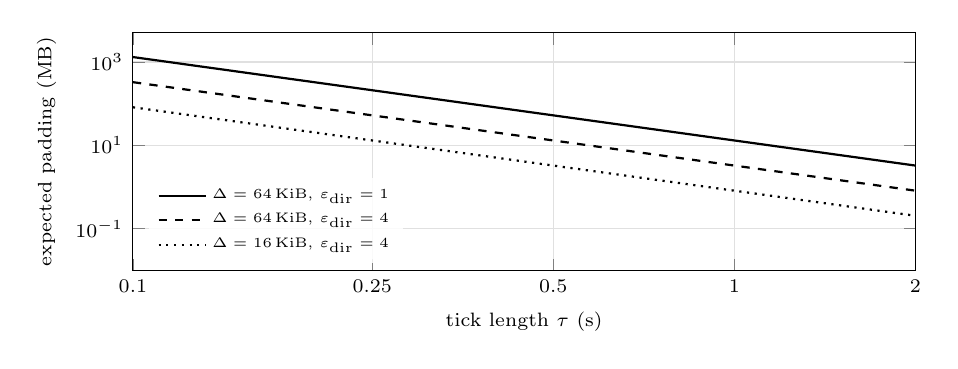
\begin{tikzpicture}
\begin{loglogaxis}[
  width=0.95\columnwidth, height=4.6cm,
  xlabel={tick length $\tau$ (s)}, ylabel={expected padding (MB)},
  xmin=0.1, xmax=2, ymin=0.01, ymax=5000,
  xtick={0.1,0.25,0.5,1,2}, xticklabels={0.1,0.25,0.5,1,2},
  legend style={font=\tiny, at={(0.02,0.03)}, anchor=south west, draw=none, fill=white, fill opacity=0.85, text opacity=1},
  tick label style={font=\scriptsize}, label style={font=\scriptsize},
  grid=major, grid style={black!12}, domain=0.1:2, samples=60]
\addplot[thick, solid] {20^2*65536/(2*x^2*1)/1e6};
\addlegendentry{$\Delta=64$\,KiB, $\varepsilon_{\mathrm{dir}}=1$}
\addplot[thick, dashed] {20^2*65536/(2*x^2*4)/1e6};
\addlegendentry{$\Delta=64$\,KiB, $\varepsilon_{\mathrm{dir}}=4$}
\addplot[thick, dotted] {20^2*16384/(2*x^2*4)/1e6};
\addlegendentry{$\Delta=16$\,KiB, $\varepsilon_{\mathrm{dir}}=4$}
\end{loglogaxis}
\end{tikzpicture}

\caption{Expected padding of the queue-length DP release per link-direction and session over a horizon $H=20$\,s, from \cref{eq:dpcost}, as a function of the tick length $\tau$, for two adjacency bounds $\Delta$ and per-direction budgets $\varepsilon_{\mathrm{dir}}$. Computed from the closed form, not measured. Plotted with PGFPlots from code prepared with AI assistance (Claude, Anthropic; see the generative AI declaration).}
\label{fig:dpcost}
\end{figure}

\begin{remark}[The exponent depends on the mechanism]\label{rem:exponent}
The quadratic growth belongs to the queue-length release with Laplace noise and basic composition, in which every tick is charged the full $\Delta$. Gaussian noise with R\'enyi DP accounting, as in NetShaper~\cite{sabzi2024netshaper}, gives, for a fixed total budget, a per-tick noise scale growing roughly like $\sqrt{K}$ (up to factors in $\log(1/\delta)$) and padding of order $K^{3/2}$. Releasing noisy \emph{arrivals} instead, $b_k=\max(0,\operatorname{round}(a_k+\mu+L_k))$ with $L_k\sim\mathrm{Lap}(\Delta/\varepsilon_{\mathrm{dir}})$ and a bias $\mu\ge0$, is $\varepsilon_{\mathrm{dir}}$-DP for the whole sequence by the Laplace mechanism on a vector with $\ell_1$ sensitivity $\Delta$; the padding per tick is at most $\max(0,\mu+L_k)$ plus half a byte, so total padding grows linearly in $K$, but the backlog is no longer bounded by the mechanism. Both variants are implemented; the completed resource evaluation uses the arrival variant and does not empirically compare the two privacy mechanisms.
\end{remark}

\begin{proposition}[Finite-horizon completion limit]\label{prop:completion}
Suppose $V\ge1$ integer bytes enter a link-direction only in its last tick, with no earlier real backlog. If the last release is $b=\max(0,\operatorname{round}(V+\mu+L))$, where $\mu\ge0$ is finite and $L\sim\mathrm{Lap}(0,s)$ with $s>0$, then
\[
 \Pr[\text{overflow}]=\tfrac12\exp\!\left(-\frac{\mu+1/2}{s}\right)>0.
\]
Thus neither finite bias in the arrivals mechanism nor the unbiased queue mechanism provides a universal zero-overflow guarantee under a fixed finite schedule that admits such arrivals.
\end{proposition}
\begin{proof}
No earlier release can serve bytes that have not arrived. The last release completes the input exactly when $b\ge V$. Apart from a probability-zero rounding tie, its complement is $L<-\mu-1/2$. The negative Laplace tail has the stated probability. Clipping at zero does not alter this event because $V\ge1$.
\end{proof}
This is a completion limit, not a refutation of the conditional release privacy statements. A deployment must declare its admissible arrivals and treatment of residual backlog; extra data-dependent sends after the horizon are outside the fixed-schedule guarantee. Empirical zero failures in a small pilot do not establish a hard reliability bound. The mechanism stress tests in \cref{sec:stress} examine this limit separately from real-network acquisition.

\begin{proposition}[Public-contract completion bound]\label{prop:contract}
On direction $j$, let integer arrivals have public total cap $V_j$, per-tick cap $A_j\le V_j$ and at most $M_j$ occupied ticks among $K_j$. They precede their tick's independent noise and arrive before the final release. In the arrivals mechanism use scale $s_j=\Delta_j/\varepsilon_j$ and finite bias $\mu_j\ge0$, optionally clipping every release to a fixed public $C_j\ge A_j$. Then
\[
 \Pr[\text{any residual backlog}]\le\sum_j\frac{M_j}{2}
       e^{-(\mu_j+1/2)/s_j}.
\]
For public $\rho_j>0$ with $\sum_j\rho_j\le\rho$, it suffices to set
\[
 \mu_j=\max\{0,s_j\log(M_j/(2\rho_j))-1/2\}.
\]
The expected application-byte release is at most
\[
 U_j=V_j+K_j\bigl[\mu_j+(s_j/2)e^{-\mu_j/s_j}+1/2\bigr],
\]
and with clipping is also bounded deterministically by $K_jC_j$.
\end{proposition}
\begin{proof}
At an occupied predictable tick, releasing fewer than its arrivals has conditional probability $p_j=\tfrac12 e^{-(\mu_j+1/2)/s_j}$. Public clipping above the arrival cap does not change this event. If it never occurs, induction leaves zero backlog after every tick. A union bound and the pathwise occupied-tick limit give $M_jp_j$ per direction, including arrivals adapted to past releases; union over directions gives the result. Also $\max(0,a+\mu+L)\le a+\max(0,\mu+L)$ for $a\ge0$, and rounding adds at most half a byte per tick. Taking expectations and summing proves $U_j$.
\end{proof}
Here $\rho$ bounds completion failure under the public arrival contract; it is not the $\delta$ of approximate DP and does not certify observable retries or aborts. Fixed clipping is output post-processing, not resampling truncated noise. The fixed-history adjacency assumptions still apply. The occupied-tick bound must be enforced at enqueue time: a streamed tool response may occupy several ticks, so counting tool calls alone is insufficient. Whole-message buffering or another justified bound is required. Late production outside the horizon remains a contract violation.

\begin{proposition}[Order of primitives]\label{prop:order}
If padding \cref{eq:pad} is applied before the DP release and the hypotheses differ in at most $n$ messages with total size at most $\Delta_0$, the padded arrival sequences differ by at most $r\Delta_0+n(\beta+1)$ bytes in $\ell_1$, so \cref{prop:dp} holds with $\Delta\ge r\Delta_0+n(\beta+1)$. If padding is applied to the released sequence instead, the guarantee of \cref{prop:dp} is unchanged and the padding adds bytes without reducing $\varepsilon$.
\end{proposition}
\begin{proof}
By \cref{prop:pad}(a) and the case $m\le\beta$, $\mathrm{pad}(m)\le\max(\beta,rm)+1\le\beta+rm+1$, where the $+1$ covers rounding to whole bytes; summing over the $n$ differing messages gives the bound. Padding the output is post-processing.
\end{proof}
The controller therefore applies rounds, then padding, then the DP release, and measures $\Delta$ directly on the bytes that enter the DP release in its calibration sessions, which satisfies \cref{prop:order} by construction.

\section{Evaluation methodology}\label{sec:eval}

The empirical scope covers implementation correctness, network resource costs, evidence preservation and a small retrospective metadata-classification diagnostic. Fixed-arrival mechanism simulations are reported separately from network measurements. The energy model and budgeted attacker-selection rule are theoretical design components. We do not test a privacy-per-joule superiority hypothesis, a server--edge comparison or a 10\,Gbps throughput claim.

\subsection{Testbed and workloads}\label{sec:testbed}
We project the public HIGGS dataset~\cite{whiteson2014higgs} to its binary label and first two input features. The source contains 11 million simulated collision records and is distributed under CC BY 4.0. The projection, site-partition order, question banks and references have separate manifests and content hashes. This reduced analytics workload is not a HIGGS classification benchmark. Four query families are used: aggregate statistics, group-by, record count and a small weighted federated-training workflow. For the latter the source bank specifies an initial step; our declared deterministic controller performs three updates, feeding the aggregate weights into the next step. We do not attribute this extension to autonomous LLM replanning.

The banks have question-, template- and cohort-separated TRAIN, SELECT and reserved final-test partitions. The calibration uses one question from each of four family and three requested-size strata, with two repetitions. Repetitions of the same question are not independent new questions. The final-test partition is not executed in this engineering study. Independent direct computation checks every aggregate update and final tool result against the same query definition without the network path.

The Mac Studio experiment runs 20 logical partitions and persistent TLS connections on one machine. Its minimal TLS RPC baseline uses the same query handler without the all-site scheduling controls. The shaped unshaped-mode baseline retains those controls. The four-instance deployment uses four \nolinkurl{m6i.2xlarge} EC2 hosts in one availability zone: T1 is the client, T2 and T3 are relays or NetShaper middleboxes, and T4 holds all 20 logical partitions. The data path uses private IP addresses. Captures at T2 and T3 observe the same TCP or QUIC/UDP segment; SSH management and evidence replication are outside that segment. This is one multiplexed observer link and one physical data endpoint, not 20 independently observed physical sites.

\subsection{Configuration selection and comparison}
The Mac TRAIN grid comprises minimal TLS, unshaped with all-site controls, fixed-1024-byte padding, bucketed padding, rounds, and DP/combined configurations with bias multipliers in $\{0,1,2,4,8\}$. The DP arrival variant uses $H=10$\,s, $\tau=0.5$\,s, a per-direction input cap of 8192 bytes and $\Delta=16384$ bytes. For $N=20$, $\varepsilon_{\mathrm{dir}}=0.2$ gives a declared session accounting budget of 8 over the 40 directions. A bias multiplier $m$ denotes $m\Delta/\varepsilon_{\mathrm{dir}}$. Rounds use $W=0.5$\,s, cover probability 1 and a 1024-byte reply frame.

We freeze the five baselines and the two cheapest fully passing TRAIN candidates from each DP family, then evaluate that shortlist on SELECT. The selected candidate in each family minimises mean framed plaintext bytes among candidates passing every SELECT trial. Truncated or incomplete trials remain failures, and host scheduling failures halt acquisition. This rule is functional/cost calibration, not \cref{alg:controller}: it uses neither an attacker score nor a calibrated joule budget. The cloud run freezes DP bias 1 and combined bias 2 from this process and evaluates seven modes: unshaped with controls, padding, rounds, DP, combined, and NetShaper with shaping disabled or enabled. It executes 12 TRAIN questions twice per mode, in a fixed seeded permutation of mode phases. We do not pool this three-step campaign with the older one-step pilot.

NetShaper~\cite{sabzi2024netshaper} runs in two middleboxes with the same client and server tools. Its resource configuration is preserved with the artifact. We do not match its privacy accounting to the tool-layer DP mechanism, so differences in byte cost cannot establish privacy superiority. The separate minimal TLS baseline is measured on Mac, not represented as an additional cloud mode.

\subsection{Model compatibility checks}
Two existing local models, \nolinkurl{mistral-small3.1:24b} and \nolinkurl{qwen2.5:14b-instruct-q4_K_M}, generate typed initial plans and structured numerical summaries. Decoding uses temperature 0, seed 20261021, an 8192-token context and at most 2048 predicted tokens. The accepted plan must match the question's reference; no fallback plan is substituted. After tool execution, the model receives the verified aggregate and must return its numerical JSON contents. Integers are exact; finite real values use relative tolerance $10^{-6}$ and absolute tolerance $10^{-8}$. Each model runs 12 TRAIN and 12 SELECT questions, with source, model and input contracts frozen before SELECT. Prompts and raw responses are retained. This measures structured-result consistency, not open-ended factual quality. The cloud workload uses a deterministic scripted controller; there is no hosted-model or LangGraph end-to-end evaluation.

\subsection{Public-contract TLS follow-up}\label{sec:localcontractmethod}
A separate exploratory Mac experiment uses three loopback TLS endpoints and generated integer tables, not the HIGGS bank or an LLM. Twelve TRAIN jobs fix planning and compute bounds at 0.04 and 0.08\,s; each bound rounds twice the observed maximum plus 0.005\,s up to a 0.04\,s multiple. The common contract has three rounds, 512/1024-byte call/reply frames and a 0.6\,s horizon. Fresh SELECT jobs use 1024 or 4096 rows per site, versus 512 on TRAIN, with scripted feedback-dependent routing. Family and round count are coupled in this pilot. Within-job policy order is randomised. The final frequency comparison freezes six or ten periodic ticks through the same horizon before dispatch. Planning/compute delays include controlled perturbations; they do not calibrate LLM bounds. Full-lifecycle loopback captures include setup, controls, ACKs and teardown. Paired-job bootstrap intervals are descriptive, conditional on this workload and host.

\subsection{Observer and privacy scope}\label{sec:attack}
The theoretical observer in \cref{sec:model} sees separate site links. The EC2 capture instead sees a multiplexed tunnel. We do not assign outer packets to logical site identities or claim measured participation privacy from that trace. A future attacker study would need observations matching the claimed threat model, retraining under each configuration, question-disjoint training and selection, a frozen final test, and question-level uncertainty estimates. The retrospective classifier in \cref{sec:retrospective} is limited to workload family and requested size on the multiplexed link; it is not a confirmatory final-test study, per-site participation attack, ROC analysis or empirical DP certification. Passing the transport and reference checks does not establish low leakage; the formal results remain conditional on their stated mechanism and deployment assumptions.

\subsection{Network metrics and evidence integrity}
Packet sizes are IPv4 lengths including TCP/UDP headers and ACKs, excluding Ethernet and the other deployment links. We use half-open per-session windows fixed by client timestamps, and separately report the full phase and bytes outside the session windows. Tool latency is measured from session start to the final tool result, including the configured 1\,s public start lead; session completion also includes any fixed covert tail. The two metrics must not be conflated with LLM answer latency or steady-state throughput.

Each capture has explicit ready and stopped timestamps and kernel-drop counters. NIC offloads are disabled for the matched capture and restored afterwards; host resources and clock offsets are screened before phases. Packet fingerprints compare both observations as an integrity diagnostic; a boundary ACK discrepancy is reported rather than silently removed. Each session has an fsync-backed intent/commit ledger and synchronous evidence replication to T4; phase results and captures are copied to Mac. Checksums, a separate controller copy and an independent restore drill protect against loss or accidental modification. Failed and superseded runs are retained under separate run identifiers, without automatic replay.

\subsection{Energy scope}\label{sec:energy}
No instance exposes an energy counter in the completed cloud testbed, and no external power meter or edge device is used. Consequently we report no measured joules, fitted per-node energy coefficients, privacy gain per joule or CO$_2$ estimate. Bytes and latency describe resource demand and do not substitute for physical energy. Calibrating \cref{eq:energy} with suitable package/DRAM counters or external instrumentation, including idle subtraction and device-specific uncertainty, remains future work~\cite{linux2026powercap}.

\subsection{Reproducibility}
The artifact records source and runtime hashes, the HIGGS projection and partition manifests, question and reference hashes, selected parameters, prompts, model responses, raw captures, per-session ledgers and cleanup records. Private SSH/TLS keys are excluded from the evidence release. The scientific implementation and public dataset licence are distinct: a release licence and public archive identifier must be supplied by the authors before submission. The completed study is descriptive; two repetitions and 12 selected questions per cloud mode do not support broad population-level or deployment-independent performance claims.

\section{Results}\label{sec:results}

\subsection{Completed engineering checks and their scope}\label{sec:engineering}
The completed preparation uses a projection of the public HIGGS data, four tool families, three contribution-size strata and 20 logical partitions. A declared deterministic controller performs three weighted federated updates for training requests, feeding each aggregate update into the next step. This is a derived workflow extension of the one-step source question bank, not evidence of autonomous multi-round agent planning. The final-test partition has not been executed.

The current implementation passes 257 software regression tests, with one optional-Torch skip. A TRAIN calibration covered 15 configurations, 12 family--size strata and two repetitions (360 trials); 349 trials passed the reference and transport-validity checks. All five baseline configurations passed their 24 trials. The zero-bias DP and combined configurations failed five and six trials, respectively; these failures are retained, rather than removed or repeated until successful. A shortlist was frozen from TRAIN before evaluating SELECT. Of 216 SELECT trials, 215 passed: the lower-bias combined candidate failed one fixed-horizon completion check. The functional/cost rule therefore selected DP bias multiplier 1 and combined bias multiplier 2. This selection minimises framed plaintext cost among the eligible candidates; it is not an empirical validation of the attacker- and energy-budget controller in \cref{alg:controller}.

\begin{table}[t]
\centering
\caption{Completed Mac engineering validation. Byte figures are mean TLS plaintext including application framing, not observed IPv4 traffic or measured energy.}\label{tab:engineering}
\footnotesize
\begin{tabular}{@{}lrr@{}}
\toprule
SELECT configuration & Passed/trials & Mean MB/session \\
\midrule
Minimal TLS RPC & 24/24 & 0.006161 \\
Unshaped with all-site controls & 24/24 & 0.337332 \\
Padding & 24/24 & 0.348878 \\
Rounds and cover sites & 24/24 & 0.376140 \\
DP, bias multiplier 1 & 24/24 & 78.184944 \\
Combined, bias multiplier 2 & 24/24 & 136.077084 \\
\bottomrule
\end{tabular}
\end{table}
The DP candidates use the arrival variant with a 10\,s horizon, 0.5\,s ticks, $\varepsilon_{\mathrm{dir}}=0.2$, an input cap of 8192 bytes and $\Delta=16384$ bytes. These functional comparisons do not establish a measured privacy gain. The difference between minimal TLS and the all-site-control baseline also shows why framing and control traffic must be reported explicitly.

Two local models, \nolinkurl{mistral-small3.1:24b} and \nolinkurl{qwen2.5:14b-instruct-q4_K_M}, each passed 12 TRAIN and 12 SELECT typed-plan, tool-result and structured numerical-summary checks in the repaired validation. Before freezing this version, each model failed two TRAIN summaries by dropping the exponent of a small coefficient. The repaired presentation supplies plain decimal JSON numbers; the numerical comparison tolerances were not relaxed, and previous failures remain archived. These 48 passing checks establish consistency for this bounded workflow, not general free-text answer quality, hosted-model robustness or autonomous replanning.

Result preservation was checked by restoring 1292 eligible files and comparing their hashes independently; calibration hashes before and after the model-only work matched. Private TLS keys were excluded from the evidence backup. No physical energy measurement, edge-device comparison, final-test attacker result or 10\,Gbps NetShaper result follows from these checks. The four-role EC2 tunnel represents one physical data endpoint and a multiplexed observer link; it does not instantiate 20 independently observed physical sites.

\subsection{Four-instance network validation}\label{sec:cloudresults}
All 168 sessions in the seven-mode, three-step-workflow campaign passed independent reference checks and transport-validity checks. Every phase committed, all 168 session replicas were acknowledged by T4, and cleanup recorded no error. Captures at both ends covered every session and reported zero kernel drops. These are functional and acquisition-validity results, not a measured privacy guarantee.

\begin{table}[t]
\centering
\caption{Four-instance EC2 validation: 24 successful sessions per mode. IPv4 bytes include headers and ACKs on the T2--T3 segment. Latency includes the public 1\,s start lead. MB denotes $10^6$ bytes.}\label{tab:cloudcost}
\footnotesize
\setlength{\tabcolsep}{3pt}
\begin{tabular}{@{}lrrr@{}}
\toprule
Mode & MB/session & Tool median (s) & Tool p95 (s) \\
\midrule
Unshaped + controls & 0.349353 & 1.123 & 1.372 \\
Padding & 0.360476 & 1.126 & 1.385 \\
Rounds & 0.392321 & 2.011 & 4.011 \\
DP (bias 1) & 78.432703 & 3.070 & 7.953 \\
Combined (bias 2) & 137.468508 & 3.575 & 9.068 \\
NetShaper disabled & 0.395938 & 1.178 & 1.593 \\
NetShaper enabled & 1.313787 & 1.313 & 1.682 \\
\bottomrule
\end{tabular}
\end{table}

\begin{figure*}[t]
\centering
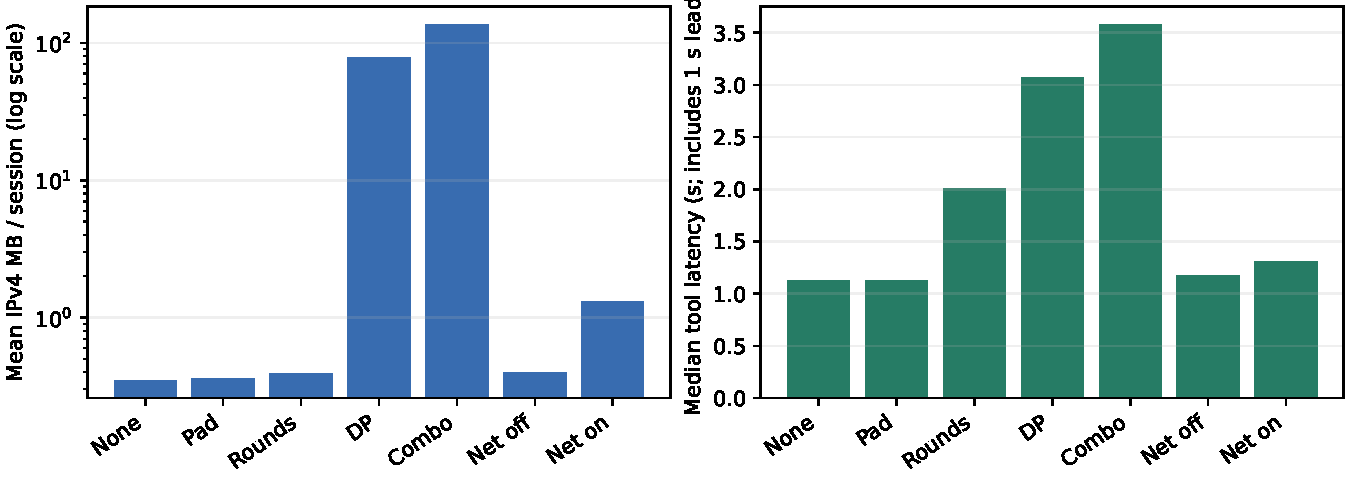
\includegraphics[width=0.94\textwidth]{audit_and_code/outputs/paper_completion_20261022/network_costs.pdf}
\caption{Observed resource costs in the descriptive EC2 campaign. The byte axis is logarithmic. These bars do not compare equal privacy or physical energy, and the seven modes ran in separate phases.}\label{fig:cloudcost}
\end{figure*}

The DP and combined configurations average 78.433 and 137.469\,MB per session on the observed link, respectively, compared with 0.349\,MB for the unshaped all-site-control baseline. Padding averages 0.360\,MB and rounds 0.392\,MB. The large DP cost remains visible after reducing the bias relative to the older pilot: it is a resource trade-off, not evidence that the selected configurations provide a better privacy--energy balance. Median fixed-horizon session completion is approximately 11\,s including the start lead, whereas the tool result can arrive earlier; the tool-latency column must not be used as the session's full protected duration.

NetShaper enabled averages 1.314\,MB within session windows, but continuous cover also exists between sessions and during setup and teardown. At T2, 31.520\,MB is outside the 24 session windows, compared with 31.531\,MB inside; the corresponding outside-window T3 count is 22.348\,MB because the full capture extents differ. We retain and report these bytes rather than equating session-window cost with deployment-wide cost. Without matched privacy accounting, the lower NetShaper byte cost cannot establish a stronger or weaker privacy guarantee.


\subsection{Retrospective cost decomposition and leakage diagnostic}\label{sec:retrospective}
We reanalyse the retained campaign without acquiring further sessions or opening the reserved final-test bank. The all-site-control baseline spends a mean 97.625\% of framed plaintext on control messages, versus 94.558\% for padding and 87.902\% for rounds. These fractions refer to application counters; they do not assign individual encrypted IPv4 packets to plaintext categories. For NetShaper enabled, 49.991\% of T2's full-capture IPv4 bytes fall outside the aligned session windows. Dividing the entire capture by its 24 sessions gives 2.627\,MB per session, compared with the in-window 1.314\,MB. This allocation includes the recorded setup and gaps and is not a steady-state estimate at arbitrary request rates.

Question-cluster bootstrap resampling (4000 draws, averaging each question's two repetitions) gives descriptive 95\% intervals of [1.025, 1.039] for the padding byte ratio, [1.085, 1.162] for rounds, [219.94, 229.08] for DP and [387.59, 398.64] for combined, relative to controls. These intervals are conditional on the acquired questions and phases; they do not remove fixed-order, host-load or temporal confounding.

We also run a fixed random-forest diagnostic using IPv4 byte and packet counts, directional bytes, packet-size statistics, inter-arrival statistics, observed packet span and 22 half-second byte bins. Labels come only from the TRAIN question manifest. Question identifiers, absolute epochs, plaintext payloads, driver tool-completion times and site identities are excluded from features. Family classification uses three leave-one-requested-size-out folds; size classification uses four leave-one-family-out folds. Both repetitions of a question remain on the same side of every split. The forest uses 100 trees, depth four, minimum leaf size two and balanced class weights, with no hyperparameter selection for this retrospective diagnostic. A byte-only forest and a majority classifier are retained as ablations.

\begin{table}[t]
\centering\footnotesize
\caption{Exploratory question-disjoint metadata classification on the multiplexed link. Each mode has only 12 questions (24 sessions). BA is balanced accuracy. Family intervals are conditional 95\% question-cluster bootstrap intervals for fixed out-of-fold predictions, excluding model-refitting uncertainty.}\label{tab:diagnostic}
\begin{tabular}{@{}lrrr@{}}\toprule
Mode & Family BA & Interval & Size BA \\\midrule
Unshaped + controls & 0.500 & [0.250, 0.708] & 0.333 \\
Padding & 0.417 & [0.208, 0.625] & 0.167 \\
Rounds & 0.583 & [0.500, 0.667] & 0.458 \\
DP & 0.292 & [0.167, 0.417] & 0.417 \\
Combined & 0.208 & [0.042, 0.375] & 0.250 \\
NetShaper disabled & 0.292 & [0.125, 0.375] & 0.375 \\
NetShaper enabled & 0.375 & [0.167, 0.583] & 0.250 \\
\midrule
Chance/majority BA & 0.250 & --- & 0.333 \\\bottomrule
\end{tabular}\end{table}

\begin{figure*}[t]\centering
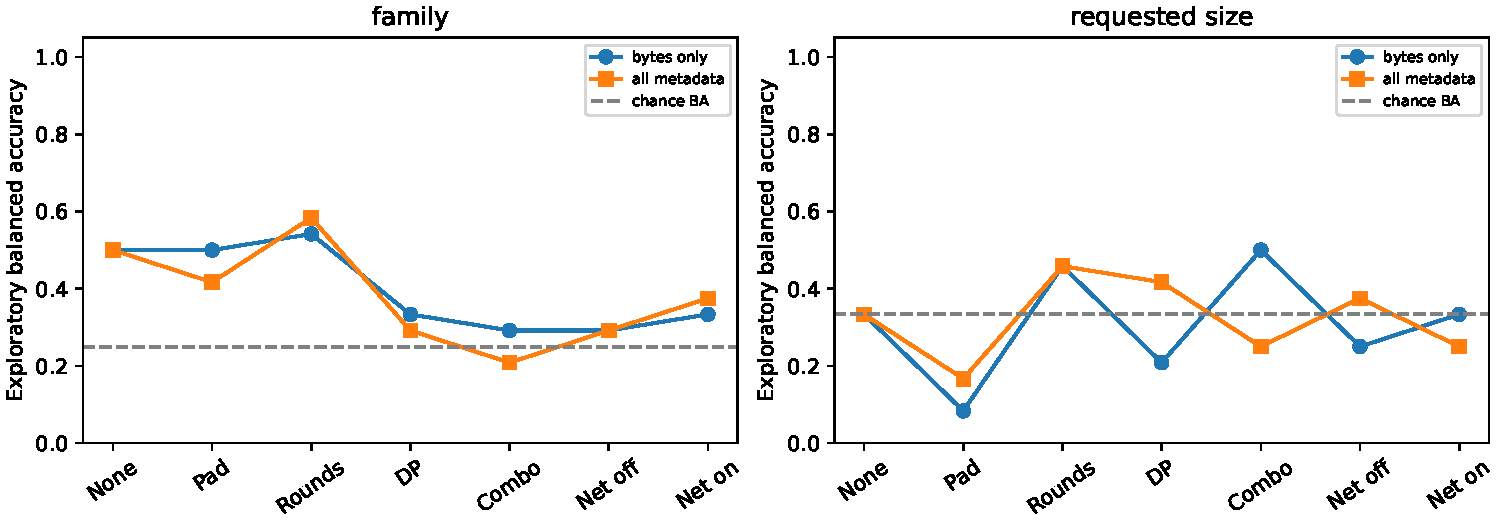
\includegraphics[width=.93\textwidth]{audit_and_code/outputs/evaluation_extension_20261022/attacker_diagnostic.pdf}
\caption{Retrospective byte-only and all-metadata random forests under question-disjoint cross-validation. Session segmentation is supplied by the retained acquisition windows. This is an exploratory diagnostic, not a final-test privacy ranking.}\label{fig:diagnostic}
\end{figure*}

Combined's family BA is 0.208 versus 0.500 for controls, whereas rounds reaches 0.583. This suggests that byte cost alone does not order the tested classifier's performance. It does not establish a privacy improvement: the small bank contains one acquired question per family--size stratum, modes occupy separate phases, and the session windows are oracle supplied rather than inferred by an observer. Requested size denotes the manifest's workload stratum, not a secret per-site contribution label. Near- or below-chance results can reflect insufficient training or distribution shift. No per-site participation result, adaptive attacker search or confirmatory final-test claim follows.

\subsection{Public-contract reliability and resource admission}\label{sec:stress}
The earlier fixed-arrival sweep (2592 cells, 128 draws each) and 90000 independent-seed checks are retained in the artifact. All three pilot-selected bias-eight configurations produced validation overflow, eight cases in total. We therefore evaluate certificates from \cref{prop:contract}, keeping the synthetic results separate from the 168 cloud sessions.

A predeclared grid has 96 synthetic deployments: $N\in\{3,10,20\}$ logical sites, $K\in\{10,20\}$ ticks, $M\in\{1,3\}$ occupied-tick caps, homogeneous or heterogeneous node profiles, total session $\varepsilon\in\{1,4\}$ and completion target $\rho\in\{0.01,0.001\}$. Each direction receives $\varepsilon/(2N)$ and $\Delta=2V$. Heterogeneous volume caps cycle through 1024, 8192 and 32768 bytes. Nonnegative weighted-byte and tick-activity costs are synthetic proxies, not joules. Budgets are constructed stress cases relative to the uniform-contract certificate, with tight and loose nodes and an additional public scaling sweep; admission rates are conditional on this design.

We compare fixed bias eight, zero-observed-failure pilot selection, a conservative $K$-tick certificate, the sharper $M$-tick certificate and per-node risk allocation. Every stochastic policy is ablated with and without a public release cap $C=V$, retaining its bias allocation across that ablation. Periodic constant cover is mandatory: it has an identical abstract frame transcript across private arrivals and is stronger than a positive-$\varepsilon$ bound in this observation model. Candidates are not selected using the new validation draws.

At the base synthetic budgets, uncapped $M$-based uniform admission succeeds in 48/96 scenarios and allocated risk in 56/96, versus 0/96 for the conservative $K$-based rule. The mean ratio of the $M$-based expected-byte upper bound to the $K$-based bound is 0.798. Allocation may increase total cost to relieve a constrained node; it is not a universal reduction in aggregate bytes. Constant cover fits all 96 cases and costs substantially less than uncapped DP in this grid. Capped DP approaches constant-cover cost. Thus the experiment does not support superiority of uncapped Laplace shaping; it identifies the importance of public caps and of a strong cover baseline.

The predeclared validation subset has 252 policy--pattern cases and 1260000 new-seed synthetic deployments with early, spread or last-tick arrivals. Four correlated pointwise 95\% intervals initially have lower limits above the mathematical bound. We retain them and freeze an additional implementation diagnostic of 200000 fresh draws for each flagged case, without changing any parameter. All four new intervals include their exact last-tick probability; the replication adds 800000 draws. These sampling checks do not prove the bound or establish empirical wire privacy. All raw flags, intervals, seeds and certificates remain available.

\begin{figure*}[t]\centering
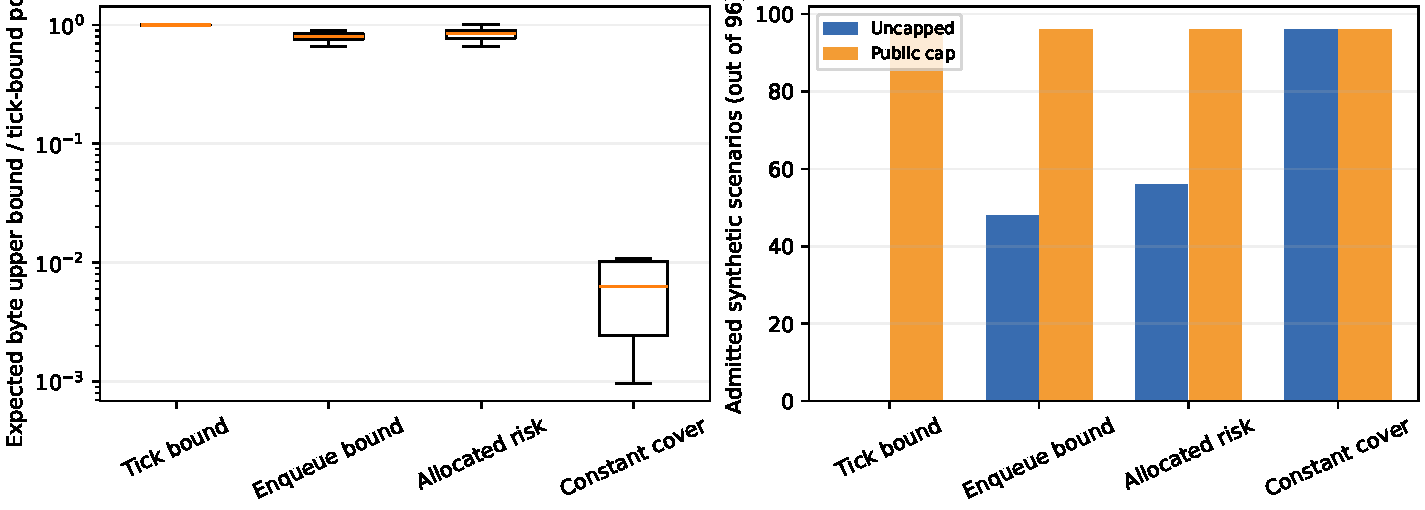
\includegraphics[width=.93\textwidth]{audit_and_code/outputs/reliability_controller_20261023/reliability_admission.pdf}
\caption{Synthetic public-contract admission. Left: distribution of expected-byte upper bounds relative to the conservative tick-count certificate. Right: base-budget admissions with and without public release clipping. Constant cover has a stronger abstract privacy certificate; no physical-energy or equal-cost superiority is inferred.}\label{fig:admission}
\end{figure*}

We separately project a public workflow envelope against periodic constant cover at identical per-direction frame caps. The 32 scenarios vary 3 or 20 logical sites, round cap 3 or 5, interval 0.1 or 0.5\,s, compute bound 0.2 or 1\,s and homogeneous or heterogeneous reply caps. Actual rounds, site participation and delays vary privately within each public envelope. There are 5000 synthetic job instances per scenario (160000 total); 1024 instances are also checked through the scalar contract implementation. A deliberately over-bound job in every scenario is rejected internally without expanding the abstract scheduled transcript. This study uses zero delivery delay; the implementation exposes a public delivery-bound parameter, but network-delay calibration is still required.

The workflow envelope uses 0.077--0.385 times the application bytes of periodic cover, a projected reduction of 61.5--92.3\%, while its projected tool p95 is 1.182--1.786 times the periodic baseline. All these byte counts are fixed by the public schedules, and both baselines have an input-independent abstract transcript. The result is a resource--latency trade-off from fewer public cover slots, not a demonstrated packet-level privacy gain or a measured system speedup. It relies on bounded planning, computation, delivery and frame volume; the current LLM and cloud acquisitions have not established those new contracts.

\begin{figure*}[t]\centering
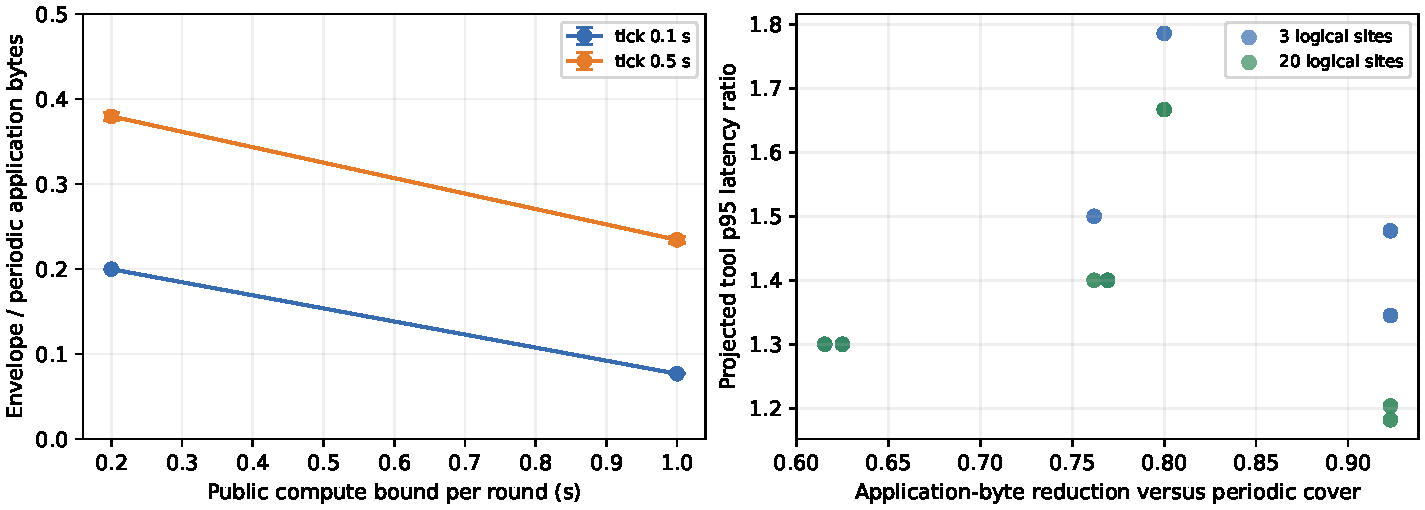
\includegraphics[width=.93\textwidth]{audit_and_code/outputs/reliability_controller_20261023/workflow_envelope_tradeoff.pdf}
\caption{Public-envelope projection against periodic constant cover: byte ratios over compute/tick bounds (left) and projected tool-p95 latency trade-offs (right). Sites are simulated, inputs stay inside declared bounds and delivery delay is zero. These are application-frame models, not EC2 wire measurements.}\label{fig:envelopetradeoff}
\end{figure*}

\subsection{Paired public-contract TLS acquisition}\label{sec:localtls}
The final local frequency comparison runs 32 new SELECT jobs under three policies (96 positive sessions) and ten deliberately invalid jobs under each (30 stress sessions). All 96 complete reference-correct within their frame and timing gates. All 30 violations---over-bound planning or computation, missed reply deadlines, and oversized calls or replies---are reported while fixed cover continues. The capture has 17054 packets, 378 connections, zero reported kernel drops and no unassigned packets; 261 evidence files pass hash checks. These are three logical sites on one physical host under recorded background load.

\begin{table}[t]\centering\small
\caption{Final paired loopback acquisition, 32 fresh scripted jobs per policy. IPv4 costs include the complete TLS lifecycle; tool completion is internal, while every public session retains the full 0.6\,s horizon.}\label{tab:localcontract}
\setlength{\tabcolsep}{5pt}
\begin{tabular}{lrrr}\toprule
Policy & Mean IPv4 (KiB) & Tool p95 (s) & Success \\
\midrule
Workflow envelope & 31.35 & 0.610 & 32/32 \\
Periodic, 6 ticks & 47.05 & 0.610 & 32/32 \\
Periodic, 10 ticks & 68.01 & 0.370 & 32/32 \\
\bottomrule\end{tabular}
\end{table}

Relative to six-tick periodic cover, the envelope's mean captured-byte ratio is 0.6662 (paired 95\% interval 0.6660--0.6664), and its tool-p95 ratio is 1.0004 (0.9986--1.0021). Against ten ticks the byte ratio is 0.461 but tool p95 is 1.649 times as long. Thus frequency choice materially changes the apparent gain: the coarser baseline reduces the saving to 33.4\%, compared with 53.9\% against ten ticks. These narrow intervals omit host and contract-selection uncertainty. Savings relative to these full-frame periodic baselines do not establish optimality over arbitrary public direction schedules or measured energy savings.

The artifact also retains an earlier phase with 63/64 positive sessions and 20/20 correctly reported stress cases: one reference-correct periodic session lost received cover frames and fails acquisition. TLS read/write operations were then serialised without blocking the sending clock on a read; a fresh-seed replication using the unchanged contract passes 64/64 positive and 20/20 stress gates. No failed run is replaced. The final frequency study uses another seed offset and keeps this repair fixed. No wire-privacy certificate, distributed-site result or empirical 0.001 completion-risk claim follows from these sample sizes.

\subsection{Capture agreement and result preservation}
Six modes match packet fingerprints exactly within the aligned session windows at both observation points. Rounds differs by two 52-byte pure ACKs at one session boundary: they are observed 20.5\,$\mu$s before the client end timestamp at T2 and 54.6--56.5\,$\mu$s after it at T3. Both ACKs are present in the full captures, whose fingerprint multisets and total byte counts match. The 104-byte window discrepancy is retained; it is not reported as payload loss or silently corrected. Clock screening and lifecycle coverage reduce acquisition ambiguity but do not eliminate timestamp-boundary sensitivity.

The compact campaign handoff was checksum-verified on the controller. All 14 raw captures were independently copied and SHA256-verified, totalling 226065099 stored pcap bytes; this storage size is distinct from the IPv4 traffic totals in \cref{tab:cloudcost}. Together with the 1292-file restore drill and unchanged calibration hashes, this provides recoverable evidence for the reported engineering results. The evidence does not include physical power measurements or a confirmatory final-test attacker evaluation.

\section{Discussion}\label{sec:discussion}

\subsection{What the analysis already implies for operators}
Four consequences of \cref{sec:analysis} hold whatever the measurements show, and they shape how the measured trade-offs should be read.
First, padding cannot hide participation or the number of rounds, because it changes neither message counts nor timing (\cref{prop:pad}). An operator who only pads protects the size of individual replies and nothing else.
Second, hiding participation has an energy floor at every site, in every session, including sites that hold nothing relevant (\cref{prop:cover}). Rounds with every site active make all links look the same within a session, but the session-level shape still depends on which sites are called. If participation is not sensitive in a deployment, cover sites can be switched off and the budget spent on size and timing. If it is sensitive, the network-wide cost grows with the number of sites, which matters most for many small edge sites.
Third, the DP release is the only primitive with a formal guarantee, and it is expensive: with the queue-length release its padding grows with the square of the number of ticks at a fixed privacy budget (\cref{eq:dpcost}), every site is active at every tick, and the guarantee needs a long-lived framed connection, a session-start signal to all sites and a fixed schedule (\cref{sec:deploy}). Releasing noisy arrivals makes padding grow only linearly in the number of ticks but leaves the backlog unbounded (\cref{rem:exponent}).
Fourth, primitives do not compose for free: padding before the DP release inflates the bytes that $\Delta$ must cover (\cref{prop:order}), so $\Delta$ has to be measured after padding.

\subsection{What the completed measurements support}
The observed cost ordering provides engineering guidance for this workload, not a privacy ranking. Padding adds modest byte cost in the tested configuration; rounds increase latency and cover traffic; fixed-tick DP release remains much more expensive in bytes, even with the lower biases chosen through functional calibration. The minimal TLS baseline shows that all-site controls account for much of the apparent unshaped baseline cost. Reporting only shaped/unshaped ratios without the control protocol would obscure this contribution.

The 168 successful EC2 sessions establish that the chosen workflow can execute through both relay and NetShaper paths under the recorded conditions. The two local models' 48 passing checks show compatibility with typed plans and structured summaries after a documented decimal-presentation repair. Neither observation establishes general agent accuracy, empirical metadata secrecy, a 10\,Gbps throughput result or measured energy savings. Resource budgets and correctness gates are useful deployment inputs, but a calibrated privacy--energy frontier requires additional measurements.

\subsection{Limitations and future work}
This is a design-and-analysis paper with bounded engineering validation. The energy coefficients remain symbolic; the four virtual machines expose no physical joule measurements. There is no edge-device study, no CO$_2$ calculation and no empirical validation of the proposed joule-budgeted controller. Bytes and active duration may inform a future energy calibration but cannot stand in for one. We therefore make no claim of privacy gain per joule or superiority at equal energy.

The formal model has separately observed site links, whereas the cloud validation has 20 logical partitions behind one physical data endpoint and a multiplexed tunnel. Its captures do not support per-site participation inference. The retrospective question-disjoint multiplexed-link diagnostic in \cref{sec:retrospective} uses a small acquired TRAIN subset; it does not replace a confirmatory attacker test, and the reserved final-test bank remains unopened. An attacker study needs a matching observer layout, retraining under each shaping configuration and frozen selection before final-test scoring. The DP theorem is conditional on its framing, cap, schedule, session-start and composition assumptions; a functioning transport alone does not certify the wire-level guarantee.

Only 12 selected question strata and two repetitions are used in each cloud mode, and mode phases are not interleaved. Time, burst capacity and execution order may confound differences. The public-data projection and hand-authored tasks do not represent all institutional workloads. The model checks use two local models and structured numerical JSON, not a hosted model, autonomous replanning or general natural-language answer quality. The cloud task driver is deterministic. Planning and final-summary traffic are outside the measured observer segment.

Packet-window agreement is sensitive to endpoint timestamp boundaries, as shown by the two ACKs in the rounds configuration. Session-window metrics exclude setup and inter-session cover, which are reported separately. The new loopback comparison instead counts the full TLS lifecycle, and shows why periodic-cover frequency must be varied. Its fixed application-frame savings remain schedule-dependent, and packet jitter is not a privacy certificate. Large-scale concurrency, distinct physical sites, instrumented power calibration and final-test attacker evaluation remain future work. The public-envelope and risk-allocation candidates still require atomic enqueue enforcement, distributed TLS lifecycle/capture integration and independent per-site wire acquisition; the synthetic and single-host results must not be presented as multi-host deployment gains. Chains of agents, compromised sites, active attacks and traffic to a hosted LLM API are outside the threat model.

\section{Conclusion}\label{sec:conclusion}
Green Shaping combines tool-layer padding, cover rounds and fixed-tick DP release with an explicit model of per-node energy budgets. Its analysis identifies limits on size protection, a participation-hiding energy floor, release privacy conditions, padding growth and finite-horizon completion limits. Public-contract bounds support a restricted resource-admission candidate, and a fixed workflow envelope exposes a conditional resource--latency trade-off. The proposed attacker- and energy-budgeted controller is a design contribution whose empirical optimum has not been established.

The completed implementation study reports functional TRAIN/SELECT calibration, 48 successful repaired local-model checks, 168 reference-correct four-instance cloud sessions, matched capture accounting and independently verified recovery. Retrospective question-disjoint classification and fixed-arrival mechanism stress tests add bounded evidence about metadata predictability and the reliability cost of finite horizons; independent-seed simulations expose failures missed by small pilot screens. The measured bytes and latency expose framing overhead and substantial DP release costs rather than demonstrating privacy or energy superiority. Preserving that distinction makes the artifact a reproducible starting point for future measurements on independently observed sites with calibrated energy instrumentation.


\section*{CRediT authorship contribution statement}
\textit{Proposed role allocation for confirmation by all authors before submission.}

\textbf{Lam Nguyen Tran Thanh:} Conceptualization, Methodology, Formal analysis, Writing -- original draft.
\textbf{Thanh Pham Chi:} Methodology, Software, Validation, Writing -- review \& editing.
\textbf{Son Ha Xuan:} Conceptualization, Supervision, Resources, Project administration, Writing -- review \& editing.
\textbf{Nguyen Ngoc Phien:} Methodology, Supervision, Validation, Project administration, Writing -- review \& editing.
\textbf{Vo Hong Khanh:} Software, Investigation, Data curation, Writing -- review \& editing.
\textbf{Nguyen Minh Triet:} Software, Formal analysis, Visualization, Writing -- review \& editing.
\textbf{Duy Pham Dang Xuan:} Investigation, Data curation, Validation, Visualization, Writing -- review \& editing.
\textbf{Tung Nguyen Quang:} Software, Investigation, Validation, Visualization, Writing -- review \& editing.

\section*{Declaration of competing interest}
The authors declare that they have no known competing financial interests or personal relationships that could have appeared to influence the work reported in this paper.

\section*{Funding}
This research did not receive any specific grant from funding agencies in the public, commercial, or not-for-profit sectors.

\section*{Acknowledgements}
We acknowledge the support of time and facilities provided by HCMC University of Technology and Engineering (HCM-UTE) for this study. This project was also undertaken with the assistance of computing resources from RACE (RMIT Advanced Computing Ecosystem).

\section*{Data availability}
The source code, de-identified packet metadata, derived evaluation data and reproducibility scripts are available in the \href{https://github.com/sonkhiemclaude-glitch/GreenShaping}{GreenShaping repository on GitHub}. The underlying HIGGS dataset is available from the UCI Machine Learning Repository under CC BY 4.0~\cite{whiteson2014higgs}; the repository supplies the source hash, projection manifest and generation code. Unredacted network captures and the reserved final-test bank are not included in this release. Reuse terms are described in the repository.

\section*{Declaration of generative AI and AI-assisted technologies in the manuscript preparation process}
During the preparation of this work, the authors used Claude (Anthropic) and Codex (OpenAI) to improve language, style and readability, and to assist with code development, analysis checks and figure preparation. The authors reviewed and edited the AI-assisted material and take full responsibility for the content of the published article.

\bibliographystyle{elsarticle-num}
\bibliography{references_verified}

\end{document}
